% Compile twice with pdfLaTeX. Figures and bibliography are included.
% Source materials: AI教練提案解析.pdf, AI_Fitness_Coach.png, A2Z outline example.pdf
\documentclass[conference]{IEEEtran}
\usepackage{amsmath,booktabs,tabularx,array,tikz,algorithmic}
\usetikzlibrary{arrows.meta,positioning}
\usepackage[hidelinks]{hyperref}
\newcolumntype{Y}{>{\raggedright\arraybackslash}X}
\tikzset{box/.style={draw,rounded corners=2pt,align=center,inner sep=4pt,font=\footnotesize},link/.style={-{Stealth[length=4pt]},thin}}
\begin{document}
\title{AI Fitness Coach: A Conversational Running Coach for Quota-Limited Cloud Deployment}
% Replace the draft label with verified author names and affiliations.
\author{\IEEEauthorblockN{Project proposal}}
\maketitle
\begin{abstract}
A runner asking whether a 30-minute outing will fit before rain arrives needs a pace calculation and a local forecast. A conversational coach must identify missing inputs, retrieve the forecast and reply while the information is still useful. We present AI Fitness Coach, a browser-based design that assigns dialogue to a single agent and delegates pace, weather, route and nutrition queries to tools. A domain filter and a usage budget constrain each turn. The interface supports spoken replies with avatar lip synchronization. The project review reports a first end-to-end demonstration on a free cloud tier. We specify a follow-up evaluation of numerical correctness, task completion, token consumption and the 95th-percentile response time for page and voice interactions. Whether the system meets the proposed latency targets under load remains open.
\end{abstract}
\begin{IEEEkeywords}
conversational agents, running, tool calling, voice interaction, latency
\end{IEEEkeywords}
\section{Introduction}
In its 2025 platform report, Strava reported a 3.5-fold increase in running clubs~\cite{strava}. Two club members can agree on a route yet need different estimates of how long it will take. A runner asking whether they can finish before the rain might omit both departure time and expected pace. A form can request both fields. A voice interface must recognize what is missing and decide which question to ask next.

AI Fitness Coach brings four tasks into one conversation: interpreting a run, computing pace, looking up weather and routes, and retrieving meal information. The project design integrates CyborAgent and CyborAssistant with a JavaScript client and FastAPI backend~\cite{project}. This paper specifies how one agent can coordinate these tasks within a quota, how to trace a reply to tool outputs, and how to measure the delay introduced by voice interaction. Section~II reviews the evidence behind these choices. Section~III describes the design. Section~IV gives the evaluation protocol, and Section~V identifies the remaining work.

\section{Related Work}
ReAct interleaves language-model decisions with observations from external tools~\cite{react}. This matters when a runner changes the requested start time after a forecast has been retrieved. The agent must recognize which observation still applies. For exercise-specific language tasks, PH-LLM used daily wearable summaries and evaluated generated coaching responses against expert assessments~\cite{phllm}. Its evaluation provides a precedent for checking the content of a reply independently of its fluency.

Running research also affects the choice of inputs. El Helou \emph{et al.} linked race-day weather to marathon finishing times across six cities~\cite{heat}. Their population-level association supports including weather context. An individual recreational runner's finish time still requires an explicit pace assumption. Table~\ref{tab:papers} connects each study to a design choice. The question for this project is whether a quota-limited service can deliver a correct calculation and a timely spoken reply when a turn also needs external data.

\begin{table*}[t]
\caption{Evidence informing the agent and the running-domain design}
\label{tab:papers}\centering\small
\begin{tabularx}{\textwidth}{@{}p{1.7cm}YYYYY@{}}\toprule
Study / year & Problem & Method & Domain knowledge & Data & Finding used here\\\midrule
ReAct~\cite{react}, 2023 & Questions requiring external evidence & Interleaved reasoning and actions & Tool selection and observation & HotpotQA, FEVER, ALFWorld, WebShop & External observations helped answer questions and guide later actions.\\
PH-LLM~\cite{phllm}, 2025 & Interpreting personal sensor summaries & Fine-tuning Gemini & Sleep and fitness coaching & Wearable summaries and 857 case studies & Experts rated fitness responses comparably to human expert responses.\\
El Helou et al.~\cite{heat}, 2012 & Relating race conditions to performance & Observational analysis & Weather and endurance running & 1,791,972 marathon finish records & Temperature had the strongest association among the weather variables studied.\\\bottomrule
\end{tabularx}
\end{table*}

\section{Proposed System}
\subsection{Architecture and turn processing}
Figure~\ref{fig:arch} shows the five components in the project materials~\cite{project}. The browser accepts text or speech. The backend exposes request--response operations over REST and carries interactive events over WebSocket. ScopeGuard checks whether a request concerns the supported fitness tasks. The agent selects a tool and interprets its output. A session snapshot carries confirmed inputs, tool results and usage into the next turn.

\begin{figure}[htbp]\centering
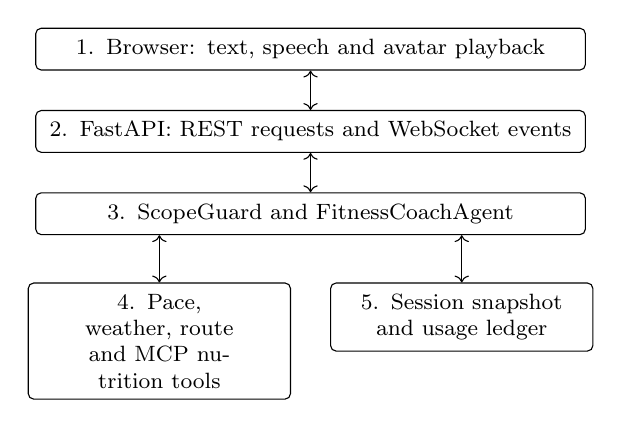
\begin{tikzpicture}[node distance=5mm]
\node[box,text width=6.7cm] (ui) {1. Browser: text, speech and avatar playback};
\node[box,below=of ui,text width=6.7cm] (api) {2. FastAPI: REST requests and WebSocket events};
\node[box,below=of api,text width=6.7cm] (agent) {3. ScopeGuard and FitnessCoachAgent};
\node[box,below=6mm of agent,xshift=-1.92cm,text width=3.05cm] (tools) {4. Pace, weather, route\\and MCP nutrition tools};
\node[box,below=6mm of agent,xshift=1.92cm,text width=3.05cm] (db) {5. Session snapshot\\and usage ledger};
\draw[<->] (ui)--(api);\draw[<->] (api)--(agent);
\draw[<->] (agent.south -| tools.north)--(tools.north);
\draw[<->] (agent.south -| db.north)--(db.north);
\end{tikzpicture}
\caption{The browser receives replies through the API. The agent accesses domain tools and persistent session state separately. MCP denotes Model Context Protocol.}\label{fig:arch}
\end{figure}

For a run with duration $t$ in minutes and distance $d>0$ in kilometres, pace is $p=t/d$ in minutes per kilometre. A 30-minute run over 5 km yields 6:00 min/km. Rounding is deferred until display. If the runner gives a number without a unit, the agent asks for the unit before saving the duration. A forecast additionally requires a place and time. Route length alone cannot resolve which forecast to use.

Figure~\ref{fig:flow} distinguishes requests that need clarification from requests ready for a tool. Algorithm~1 specifies a proposed accounting rule. Before a billable call, reserve an upper bound $r$ on its token cost. If actual usage is $u\leq r$, release $r-u$ tokens. With starting balance $B$, the resulting balance is $B-u$. A timeout with unknown usage keeps its reservation until reconciliation. Atomic reservations prevent two turns from spending the same balance.

\begin{figure}[htbp]\centering
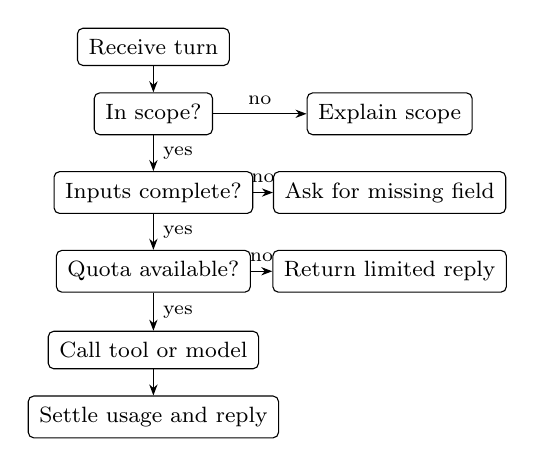
\begin{tikzpicture}
\node[box] (input) at (0,0) {Receive turn};
\node[box] (scope) at (0,-.85) {In scope?};
\node[box] (fields) at (0,-1.85) {Inputs complete?};
\node[box] (budget) at (0,-2.85) {Quota available?};
\node[box] (work) at (0,-3.85) {Call tool or model};
\node[box] (reply) at (0,-4.7) {Settle usage and reply};
\node[box] (redirect) at (3,-.85) {Explain scope};
\node[box] (ask) at (3,-1.85) {Ask for missing field};
\node[box] (stop) at (3,-2.85) {Return limited reply};
\draw[link] (input)--(scope);
\foreach \a/\b in {scope/fields,fields/budget,budget/work}{\draw[link] (\a)--node[right,font=\scriptsize]{yes}(\b);}
\foreach \a/\b in {scope/redirect,fields/ask,budget/stop}{\draw[link] (\a)--node[above,font=\scriptsize]{no}(\b);}
\draw[link] (work)--(reply);
\end{tikzpicture}
\caption{Decision path for one turn. Each right-hand branch returns control to the runner.}\label{fig:flow}
\end{figure}

\par\smallskip\noindent\textbf{Algorithm 1. Processing a coaching turn}
\begin{algorithmic}[1]
\STATE Load the snapshot and any completed reply for the turn ID.
\IF{the turn already has a completed reply}
  \STATE Return the stored reply.
\ENDIF
\STATE Apply ScopeGuard. Return guidance if outside scope.
\STATE Resolve units, place and time required by the intent.
\IF{a required field is missing}
  \STATE Save the pending intent, ask for the field and end turn.
\ENDIF
\FOR{each required call, up to the turn limit}
  \STATE Reserve its cost bound atomically or return a quota notice.
  \STATE Invoke the call and record the result or error.
  \STATE Settle known usage or flag the reservation for reconciliation.
  \IF{enough evidence is available, or a required call failed}
    \STATE Exit loop.
  \ENDIF
\ENDFOR
\STATE Save the evidence and reply under the turn ID.
\STATE Return text and, when requested and available, speech.
\end{algorithmic}

\subsection{Design tradeoffs}
Five principles guide the design: preserve units in arithmetic, identify the time and place of each forecast, trace factual claims to tool results, reserve scarce resources before use, and retain enough state to resume interrupted turns. Three choices expose tensions between these principles. Free-form input reduces the number of fields a runner must navigate but can omit units, so clarification precedes arithmetic. A single agent avoids handoffs but shares context across tasks, so each tool receives only the fields it needs. Streaming audio shortens the perceived wait but can speak an obsolete estimate, so the client waits for required evidence before playing a numerical answer.

\section{Evaluation Protocol}
The project review reports that a first-stage demonstration completed a conversation, weather and route lookup, nutrition interaction and lip-synchronized reply on a free cloud tier~\cite{project}. It supplies no turn-level logs, sample counts or latency distribution. Stage two therefore uses the following prospective protocol.

\subsection{Comparisons and measurement}
Run the same tasks through a form interface, the cloud agent and a local deployment of the same agent. For both agent deployments, fix the model, prompts, tool responses and token cap where possible. Test live services separately to expose network variation. Compare all three on field accuracy and task completion. Compare voice onset across voice-capable configurations. Report cold starts separately from warm turns, and retain failed turns in the completion denominator.

As a starting point, repeat each scenario at least 30 times per configuration and publish the sample count. Time page queries from submission to visible data, and voice turns from the end of user speech to the first audible reply. For $n$ successful trials, sort durations and report the observation at rank $\lceil0.95n\rceil$, alongside timeout and failure counts. The proposed targets are page-query P95 below 2~s and voice-onset P95 below 12~s. Record tokens per completed task, clarification turns and the fraction of factual replies supported by tool results. Vary the token cap and concurrency to identify when either latency target fails.

\subsection{Ten questions for validating the coach}
Each question has an observable answer for a scripted test.
\begin{enumerate}
\item What pace follows from 5 km in 30 min? The expected value is 6:00 min/km.
\item How is zero distance handled? The client requests a positive distance and displays no pace.
\item What happens when units are omitted? The next turn asks for the unit and preserves the number.
\item Which forecast fits a changed departure time? Its validity interval must cover the updated time at the requested location.
\item What if a route lookup times out? The reply identifies the missing route and omits its length.
\item Where did a meal estimate come from? The trace links it to an MCP result and its portion size.
\item Does an unrelated request use a domain tool? The trace ends at ScopeGuard before such a call runs.
\item Can concurrent turns exceed the balance? Settled usage plus active reservations must stay within the starting quota.
\item Does reconnecting duplicate a completed turn? Resubmitting its ID returns the stored reply and leaves the ledger unchanged.
\item When does the avatar respond? Record the offset between first audible speech and first mouth motion separately from voice onset.
\end{enumerate}
Unit tests cover arithmetic and budget updates. Integration tests inject stale forecasts, timeouts and duplicate turn IDs. A browser smoke test exercises spoken input through audio playback. A separate study with runners would be needed to evaluate usability or sustained training effects.

\section{Conclusion}
AI Fitness Coach combines a conversational interface with explicit pace calculation, time-specific weather and route lookup, and nutrition retrieval. The next empirical step after the reported demonstration is to publish turn-level measurements showing which tasks meet the response-time targets and where quota limits interrupt a conversation. Phone GPS traces, step counts and posture sensing remain future extensions. Each would need its own validation before it could inform coaching replies.

\begin{thebibliography}{00}
\bibitem{strava} Strava, \emph{12th Annual Year in Sport Trend Report}, Dec. 3, 2025. \href{https://press.strava.com/en-gb/articles/strava-releases-12th-annual-year-in-sport-trend-report-2025}{Online report}.
\bibitem{project} \emph{AI Fitness Coach Proposal Analysis}, course project review, pp. 1--2, undated, in Chinese. Supplied with the project infographic.
\bibitem{react} S. Yao \emph{et al.}, \textquotedblleft ReAct: Synergizing reasoning and acting in language models,\textquotedblright\ in \emph{Proc. Int. Conf. Learning Representations}, 2023. \href{https://react-lm.github.io/}{Project and paper}.
\bibitem{phllm} J. Khasentino \emph{et al.}, \textquotedblleft A personal health large language model for sleep and fitness coaching,\textquotedblright\ \emph{Nature Medicine}, vol. 31, pp. 3394--3403, 2025, \href{https://doi.org/10.1038/s41591-025-03888-0}{doi: 10.1038/s41591-025-03888-0}.
\bibitem{heat} N. El Helou \emph{et al.}, \textquotedblleft Impact of environmental parameters on marathon running performance,\textquotedblright\ \emph{PLOS ONE}, vol. 7, no. 5, Art. no. e37407, 2012, \href{https://doi.org/10.1371/journal.pone.0037407}{doi: 10.1371/journal.pone.0037407}.
\end{thebibliography}
\end{document}

